 
% !TeX spellcheck = pl_PL
\documentclass[]{article}
\usepackage[polish]{babel}
\usepackage[utf8]{inputenc}
\usepackage[T1]{fontenc}
\usepackage{array}
\usepackage{amsmath}
\usepackage{graphicx}
\usepackage{multirow}
\usepackage{makecell}
\usepackage{geometry}
\graphicspath{{./images/}}


\newgeometry{vmargin={30mm}, hmargin={30mm}}
	\begin{document}
		\begin{table}[h]
		\centering
		\begin{tabular}{|c|c|c|c|c|c|}
			\hline 
			\makecell{Nr. \\ ćwicz.}& \makecell{Data} & \makecell{Imię i nazwisko} & \makecell{Wydział} & \makecell{Semestr} & \makecell{Grupa I1\\nr. lab.} \\ 
			121 & 29 listopada 2019 & \makecell{Jakub Gosławski 141222\\Michał Wiśniewski 141355} & Informatyki & 3 & 5 \\ 
			\hline 
			\multicolumn{3}{|l|}{Prowadzący: Wojciech Marciniak} &  &  \multicolumn{2}{l|}{Ocena:}  \\
			\hline
		\end{tabular}
	\end{table} 

	Temat ćwiczenia: Badanie rezonansu mechanicznego
	
	\section{Podstawy Teoretyczne}
	Rodzaj ruchu, jaki wykonuje ciało, jest określony przez własności siły na nie działającej. Ruch nazywamy harmonicznym, jeżeli siła działająca na ciało jest skierowana do jednego punktu, będącego położeniem równowagi i jej wartość jest proporcjonalna do wychylenia ciała z położenia równowagi.\\
	Układ fizyczny posiadający powyższe własności nazywamy oscylatorem harmonicznym.\\
	W rozważanym w tym zadaniu przykładzie mamy doczynienia z ruchem harmonicznym prostym, ponieważ działają tylko siły sprężystości.
	\subsection{Wzory}
	\begin{align}
	\beta = \frac{1}{T}ln\frac{A_n}{A_{n+1}}\\
	\omega_0 = \frac{2\pi}{T}\\
	\omega '=\sqrt{\omega^2_0 = \beta^2}\\
	\tau = \frac{1}{2\beta}\\
	Q = \omega_0\tau = \frac{\omega_0}{2\beta}
	\end{align}
	(1) wspólczynnik wytłumienia
	(2,3) częstotliwość kołowa
	(4) czas relaksacji
	(5) dobroć oscylatora
	\section{Wyniki Pomiarów i  Obliczenia}
	\subsection{Elektromagnes $0V$}
	Zmierzony czas 10 wachnięć - $17.01s$\\
	Okres $T = \frac{17.01s}{10}=1.70s$\\
	$\omega = 3.69 \left[ \frac{rad}{s}\right]$\\
	$\omega' = 3.69 \left[ \frac{rad}{s}\right]$\\
	Ponieważ dla tej wartości napięcia w elektromagnesie wartość $\beta$ jest tak mała że po zaokrągleniu $\omega=\omega'$\\
	Zmierzone amplitudy kolejnych wachnięć i obliczone współczynniki tłumienia
	\begin{table}[h]
		\begin{tabular}{|c|c|}
			\hline 
			A[cm] & $\beta\left[ \frac{1}{s}\right] $ \\ 
			\hline 
			18.0 & 0.00657 \\ 
			\hline 
			17.8 & 0.00664 \\ 
			\hline 
			17.6 & 0.00672 \\ 
			\hline 
			17.4 & 0.00680 \\ 
			\hline 
			17.2 &  \\ 
			\hline 
		\end{tabular} 
	\end{table}

	$\beta_{\text{śr}} = 0.00668 \left[ \frac{1}{s}\right] $
	
	$\tau=74.83[s]$
	
	$Q = 276.41$
	
	\newpage
	\subsubsection{Drgania wymuszone}
	
	\begin{table}[h]
		\centering
		\caption{Pomiary Amplitudy i czasu 10 wachnięć dla różnych wartości natężenia prądu w silniku}
		\begin{tabular}{|l|l|l|l|l|}
			\hline
			
			I [A] & 10t [s] & A [cm] & T [s] & $\omega'$ [1/s] \\ \hline
			5 & 27.76 & 1 & 2.776 & 2.263 \\ \hline
			5.5 & 24.35 & 1 & 2.435 & 2.580 \\ \hline
			6 & 22.25 & 1.6 & 2.225 & 2.824 \\ \hline
			6.5 & 20.86 & 2.6 & 2.086 & 3.012 \\ \hline
			7 & 18.64 & 4 & 1.864 & 3.371 \\ \hline
			7.5 & 17.61 & 16.2 & 1.761 & 3.568 \\ \hline
			8 & 16.12 & 5.4 & 1.612 & 3.898 \\ \hline
			8.5 & 15.57 & 3.2 & 1.557 & 4.035 \\ \hline
			9 & 14.99 & 1.4 & 1.499 & 4.192 \\ \hline
			9.5 & 13.93 & 1.2 & 1.393 & 4.511 \\ \hline
			10 & 13.26 & 1 & 1.326 & 4.738 \\ \hline
			
		\end{tabular}
	\end{table}
	
	Częstotliwość rezonansowa:
	$$\omega = 3.568 \left[ \frac{rad}{s}\right]$$\\
	Całkowita szerokość rezonansu:
	$$2\Delta\omega_{\frac{1}{2}} = 0.0134 \left[ \frac{1}{s}\right] $$\\	
	Dobroć oscylatorowa wyliczona ze wzoru (5):
	$$Q = 276.41$$
	
	
	\subsection{Elektromagnes $10V$}
	Zmierzony czas 10 wachnięć - $17.49s$\\
	Okres $T=\frac{17.49s}{10} = 1.75s$\\
	$\omega = 3.59 \left[ \frac{rad}{s}\right]$\\
	$\omega' = 3.59 \left[ \frac{rad}{s}\right]$\\
	Zmierzone amplitudy kolejnych wachnięć i obliczone współczynniki tłumienia
	\begin{table}[h]
		\begin{tabular}{|c|c|}
			\hline 
			A[cm] & $\beta\left[ \frac{1}{s}\right] $ \\ 
			\hline 
			18.0 & 0.112 \\ 
			\hline 
			14.8 & 0.191 \\ 
			\hline 
			10.6 & 0.175 \\ 
			\hline 
			7.8 & 0.189 \\ 
			\hline 
			5.6 &  \\ 
			\hline 
		\end{tabular} 
	\end{table}

	$\beta_{\text{śr}} = 0.167 \left[ \frac{1}{s}\right] $
	
	$\tau=2.996[s]$
	
	$Q = 10.76$
	
	\subsubsection{Drgania wymuszone}
	
	\begin{table}[h]
		\centering
		\caption{Pomiary Amplitudy i czasu 10 wachnięć dla różnych wartości natężenia prądu w silniku}
		\begin{tabular}{|l|l|l|l|l|}
			\hline
			
			I [A] & 10t [s] & A [cm] & T [s] & $\omega'$ [1/s] \\ \hline
			5 & 26.68 & 0.8 & 2.668 & 2.349 \\ \hline
			5.5 & 24.13 & 1.2 & 2.413 & 2.599 \\ \hline
			6 & 22.08 & 1.2 & 2.208 & 2.841 \\ \hline
			6.5 & 20.17 & 1.8 & 2.017 & 3.111 \\ \hline
			7 & 19.2 & 2.8 & 1.92 & 3.268 \\ \hline
			7.5 & 17.41 & 4.8 & 1.741 & 3.605 \\ \hline
			8 & 16.45 & 2.2 & 1.645 & 3.816 \\ \hline
			8.5 & 15.32 & 1.6 & 1.532 & 4.098 \\ \hline
			9 & 14.4 & 1 & 1.44 & 4.360 \\ \hline
			9.5 & 14.12 & 0.8 & 1.412 & 4.447 \\ \hline
			10 & 13.08 & 0.6 & 1.308 & 4.801 \\ \hline
			
		\end{tabular}
	\end{table}
	
	Częstotliwość rezonansowa:
	$$\omega = 3.605 \left[ \frac{rad}{s}\right]$$\\
	Całkowita szerokość rezonansu:
	$$2\Delta\omega_{\frac{1}{2}} = 0.334 \left[ \frac{1}{s}\right] $$\\	
	Dobroć oscylatorowa wyliczona ze wzoru (5):
	$$Q = 10.76$$
	
	\subsection{Elektromagnes $10V$}
	Zmierzony czas 3 wachnięć - $5.33s$, po 3 wachnięciach wachadło zatrzymało się\\
	Okres $T=\frac{5.33s}{3} = 1.77s$\\
	$\omega = 3.53 \left[ \frac{rad}{s}\right]$\\
	$\omega' = 3.43 \left[ \frac{rad}{s}\right]$\\
	Zmierzone amplitudy kolejnych wachnięć i obliczone współczynniki tłumienia
	\begin{table}[h]
		\begin{tabular}{|c|c|}
			\hline 
			A[cm] & $\beta\left[ \frac{1}{s}\right] $ \\ 
			\hline 
			18.0 & 0.582 \\ 
			\hline 
			6.4 & 0.655 \\ 
			\hline 
			2.0 & 0.1.296 \\ 
			\hline 
			0.2 &  \\ 
			\hline 
		\end{tabular} 
	\end{table}
	
	$\beta_{\text{śr}} = 0.844 \left[ \frac{1}{s}\right] $
	
	$\tau=0.592[s]$
	
	$Q = 2.09$
	
	\subsubsection{Drgania wymuszone}
	
	\begin{table}[h]
		\centering
		\caption{Pomiary Amplitudy i czasu 10 wachnięć dla różnych wartości natężenia prądu w silniku}
		\begin{tabular}{|l|l|l|l|l|}
			\hline
			
			I [A] & 10t [s] & A [cm] & T [s] & $\omega'$ [1/s] \\ \hline
			5 & 26.59 & 0.8 & 2.659 & 2.207 \\ \hline
			5.5 & 24.14 & 0.8 & 2.414 & 2.462 \\ \hline
			6 & 22.05 & 1 & 2.205 & 2.722 \\ \hline
			6.5 & 20.57 & 1.2 & 2.057 & 2.936 \\ \hline
			7 & 18.59 & 1.2 & 1.859 & 3.273 \\ \hline
			7.5 & 17.46 & 1.4 & 1.746 & 3.498 \\ \hline
			8 & 16.19 & 1.2 & 1.619 & 3.788 \\ \hline
			8.5 & 15.33 & 1 & 1.533 & 4.011 \\ \hline
			9 & 14.35 & 0.8 & 1.435 & 4.296 \\ \hline
			9.5 & 13.61 & 0.6 & 1.361 & 4.539 \\ \hline
			10 & 13.07 & 0.6 & 1.307 & 4.733 \\ \hline
			
			
		\end{tabular}
	\end{table}
	
	Częstotliwość rezonansowa:
	$$\omega = 3.498 \left[ \frac{rad}{s}\right]$$\\
	Całkowita szerokość rezonansu:
	$$2\Delta\omega_{\frac{1}{2}} = 1.689 \left[ \frac{1}{s}\right] $$\\	
	Dobroć oscylatorowa wyliczona ze wzoru (5):
	$$Q = 2.09$$
	
	\section{Dyskusja Błędów Pomiarowych}
	Ponieważ nie można było zatrzymywać wahadła aby dokonać dokładnego pomiaru, pomiary musiały być wykonywane dość nieprecyzyjnie, ze względu na brak precyzji ludzkiego oka i refleksu.\\
	Same niepewności pomiarowe wynosiły odpowiednio 0.01s dla stopera i 0.2 cm dla podziałki amplitudy.\\
	Z powodu znaczącej ale trudnej do zdefiniowania niepewności wynikającej z błędu ludzkiego, jest ona pomijana
	\section{Wnioski}
	Niezależnie od siły wyhamowującej działającej na ciało jego częstotliwość rezonansowa pozostaje stała, co można odczytać z wykresów
	\section{Wykresy}
	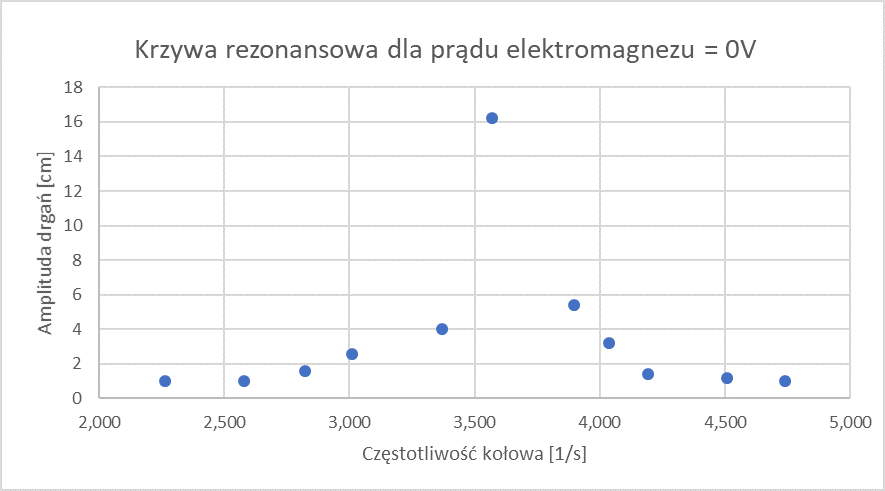
\includegraphics[width=\linewidth]{wykres1}
	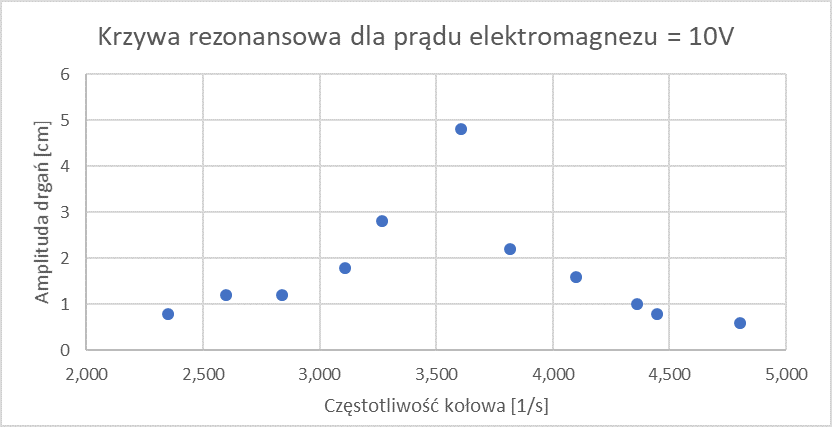
\includegraphics[width=\linewidth]{wykres2}
	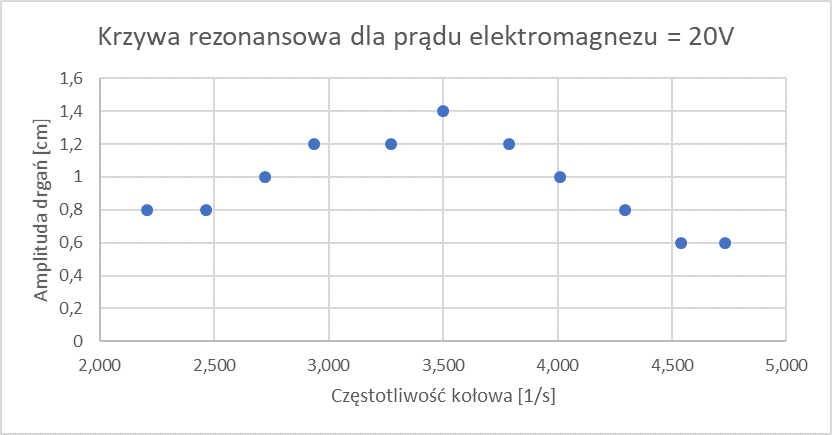
\includegraphics[width=\linewidth]{wykres3}
\end{document}